\documentclass{article}

\textwidth=6.5in
\textheight=8.5in
\voffset=-54pt
\oddsidemargin=0in
\evensidemargin=0in
\setlength{\parskip}{8pt}
\setlength{\parindent}{0pt}

\usepackage{amsmath, amssymb}
\usepackage{ifthen}

\usepackage[inline]{enumitem}
\setlist{topsep=0pt, parsep=8pt}

\usepackage[rgb,table]{xcolor}\convertcolorsUfalse
\usepackage{graphicx}

% change hyperref options
\PassOptionsToPackage{hyphens}{url}
\usepackage[bookmarks,colorlinks,linkcolor=black,citecolor=blue,pdfstartview=FitH,urlcolor=blue]{hyperref}
\hypersetup{pdfpagemode=UseNone}
\usepackage{bookmark}

\usepackage{graphicx}
\usepackage{multicol}
\usepackage{framed}
\usepackage{array}

\usepackage{icomma}

\usepackage{soul}
\usepackage[normalem]{ulem}

\usepackage{pgfplots}
\pgfplotsset{compat=1.18}  
\pgfplotscreateplotcyclelist{mycolor}{black, blue, red, green!70!black, magenta, purple, cyan, orange }  
\pgfplotsset{
  disabledatascaling,
  cycle list=tikzcolor, 
  axis lines=middle,
  every axis plot/.style={no marks, thick},
  every axis/.style={
    enlarge x limits=false,
    enlarge y limits=auto,
    xlabel style={at={(current axis.right of origin)},anchor=west},
    ylabel style={at={(current axis.above origin)},anchor=south},
    % extra x and y ticks for asymptotes
    extra x tick style={grid=major, grid style={dashed,black}},
    extra y tick style={grid=major, grid style={dashed,black}},
    /pgf/number format/1000 sep={},
  },    
  tick label style = {font=\footnotesize, fill=\currentbgcolor, inner sep=0pt},    
  xticklabel shift=1pt,    
  scaled ticks=false,
  scaled y ticks=false,
  unbounded coords=jump,
  samples=101,
  minor tick length=0,
  scatter/classes={
    open={mark=*,draw=black,fill=white, mark size=2, thin},
    closed={mark=*,draw=black,fill=black, mark size=2, thin}
  },
  width=3in,
}
\pgfplotsset{open/.style={only marks, mark=*, fill=white, thin, mark size=2}}
\pgfplotsset{closed/.style={only marks, mark=*, draw=black, fill=black,
    thin, mark size=2}}
\pgfplotsset{labeled/.style={nodes near coords, only marks, mark=*, draw=black, fill=black, thin, mark size=2, point meta=explicit symbolic}}

\usepackage{tikz}
\usetikzlibrary{
  matrix,%
  % enables the snake paths
  decorations.pathmorphing,%
  % enables bigger arrows
  decorations.markings,%
  decorations.pathreplacing,%
  decorations.text,%
  calc,%
  patterns,%
  shapes.geometric,%
  arrows,
  decorations.shapes,
  positioning,
  plotmarks,
  intersections
}
\tikzset{>=latex} % sets default arrow type in tikz
\tikzset{font=\normalsize}
\tikzset{mark size=1.5pt, mark options=thin}
\tikzset{pin distance=4pt,
  every pin edge/.style={<-, thin, shorten <= -2pt}}
  \usepackage{setspace}

\interfootnotelinepenalty=10000
\renewcommand{\thefootnote}{(\arabic{footnote})}

\usepackage{multirow, bigdelim}

% change to \usepackage[sols]{handout} to see solutions
\usepackage[]{handout}

\newcommand\iscurrentenumi[1]{%
  \ifthenelse{\equal{#1}{\theenumi}}{}{#1}}
\setenumerate[1]{ref=\#\arabic*}
\setenumerate[2]{ref=\protect\iscurrentenumi{\theenumi}(\alph*)}
\newcommand\enumiiprefix[2]{%
  \ifthenelse{{\equal{#1}{\theenumi}}\AND{\equal{#2}{(\alph{enumii})}}}{}{}%
  \ifthenelse{{\equal{#1}{\theenumi}}\AND{\NOT{\equal{#2}{(\alph{enumii})}}}}{#2}{}%
  \ifthenelse{\equal{#1}{\theenumi}}{}{#1#2}%
}
\setenumerate[3]{ref=\protect\enumiiprefix{\theenumi}{(\alph{enumii})}\roman*}

\newlength{\tipmargin}
\makeatletter

% underline links               
\let\@href=\href
\renewcommand{\href}[2]{\@href{#1}{\ul{#2}}}

\renewenvironment{framed}{
  \setlength{\tipmargin}{\textwidth-\linewidth}
  \advance\@totalleftmargin-\tipmargin
  \def\FrameCommand{\hspace{\tipmargin}\fbox}%
  \advance\linewidth\tipmargin
  \MakeFramed {\advance\hsize-\width \FrameRestore}%
}
{\endMakeFramed}

\makeatother

\definecolor{purple}{rgb}{0.5,0,1.0}
\definecolor{hotpink}{rgb}{1, 0, 0.5}

\definecolor{skyblue}{rgb}{0, 0.5, 1}

\newcommand{\robin}{\href{https://people.math.harvard.edu/~jjchen/mathma/docs/handouts/Gottlieb.html}{Gottlieb}}

\newcounter{imagecounter}
\newcounter{columncounter}
\newenvironment{imagetable}[3][]{%
  \setcounter{imagecounter}{0}
  \setcounter{columncounter}{#2}
  \addtocounter{columncounter}{-1}
  \newcolumntype{i}{>{\raisebox{-1ex-\height}{\makebox[1em]{\hfill\stepcounter{imagecounter}(#3{imagecounter})}}\hspace{4pt}\begin{minipage}[t]{\linewidth/#2-1em-\tabcolsep*3}\arraybackslash\vspace{0pt}}l<{\end{minipage}}}
\begin{tabular}{i*{\value{columncounter}}{#1i}}}
{\end{tabular}}  

\usepackage{fancyhdr}
\lhead{\textcolor{white}{This content is protected and may not be shared, uploaded, or distributed.}}
\rhead{}
\rfoot{\vspace*{\fill}\footnotesize\textcopyright{} \emph{Harvard Math Ma}}
\renewcommand{\headrulewidth}{0pt}
\pagestyle{fancy}
\begin{document}

\htitle{1: Introduction to Functions}

  \begin{problemonly}
    $\bigstar$ \emph{Reminders:}
    \begin{itemize}
    \item If you haven't take the Ma/1a skill check, you will want to do that right away. Make sure to email our course head, Kate Penner at penner@math.harvard.edu if you haven't yet.
    \item If you haven't already, please sign up for Edfinity Math Ma 2024 ASAP after class to make sure it works on your device. It will host part of your homework assignment due at our next class!
    \item Purchase your workbook at Flashprint as soon as possible if you haven't already!
    \item Workshop time preferences are due today. They will run Tuesdays, beginning next week, Tuesday, September 10.
    \end{itemize}

    \begin{center}
      \rule{5in}{0.4pt}
    \end{center}

    This worksheet is your personal guide to the material we cover in class. As you work through the problems, take some time to write down the key points you want to take away from class.

    We intentionally make these worksheets too long to finish in class so that you'll always have some extra practice problems. Each section may cover different problems to cover learning objectives; we'll post solutions on the course website after class. 

    Each day, we'll list some learning objectives. Here are today's: 
  \end{problemonly}

\begin{problemonly}
  \begin{framed}

You should be able to:

    \item Explain what a \emph{function} is, and distinguish between
      functions and non-functions.

    \item Identify the \emph{independent variable}, \emph{dependent
        variable}, \emph{domain}, and \emph{range} of a function.

    \item Explain how slope graphically represents a rate of change.

    \item Reason about whether a function is \emph{increasing} or
      \emph{decreasing}, as well as whether it's \emph{concave up}, 
      \emph{concave down}, or \emph{linear}.

    \end{itemize}
  \end{framed}
\end{problemonly}

\begin{problemonly}
  The learning objectives should give you an idea of the basic skills
  and concepts from each day that we expect you to be comfortable
  with. Class will introduce you to these ideas, but the pset is where
  you'll really get comfortable with them! After you finish the pset, 
  take a look back at the learning objectives, and check how you're
  feeling about them. If you don't feel comfortable with an objective, 
  we encourage you to stop by MQC or office hours to talk about it
  more.
\end{problemonly}

\pspace{\newpage}

\begin{enumerate}
\item   \label{function-football}

  \begin{enumerate}
  \item \label{function-football-pass}

    \note{Here, the key useful feature to think about ends up being
      whether the function is increasing or decreasing. When we go
      over this, I will highlight the words \emph{increasing} and
      \emph{decreasing}.} 

    \begin{problem}
      During a football game at Harvard Stadium, the quarterback stands at the 50-yard line (right in the middle of the field) and throws the ball to a receiver near the end of the field marked \textsc{crimson}.

      % picture from
      % https://moneywise.com/a/ch-c/worst-stadiums-in-college-football_november2018/p-6?t=These+Are+The+Worst+College+Football+Stadiums
      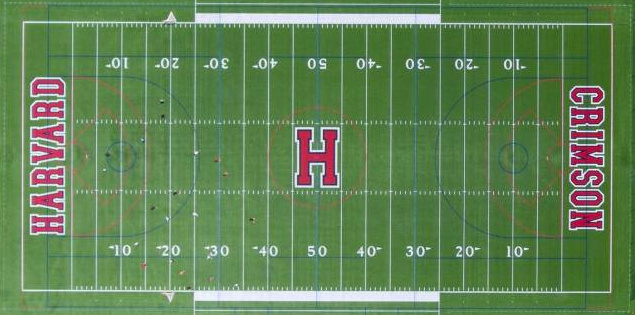
\includegraphics[width=3.5in]{images/harvard-stadium-cropped.jpg}

      3 seconds after the quarterback releases the ball, the receiver catches the ball at the 10-yard line (which is labeled 10 in the picture). One of the following graphs shows the ball's horizontal position (which yard line it's at) while it's in the air. Which one?
    \end{problem}

    \begin{imagetable}{2}{\Alph}
      \begin{tikzpicture}
        \begin{axis}[enlarge x limits=auto, ymin=0, xlabel style={align=center}, xlabel={time\\(seconds)}, ylabel={position\\(yard line)}, ylabel style={align=center}, xtick=\empty, ytick=\empty, width=2.25in]
          \addplot[domain=0:3] { 10 + 40/3 * x};
        \end{axis}
      \end{tikzpicture} & 
      \begin{tikzpicture}
        \begin{axis}[enlarge x limits=auto, ymin=0, xlabel style={align=center}, xlabel={time\\(seconds)}, ylabel={position\\(yard line)}, ylabel style={align=center}, xtick=\empty, ytick=\empty, width=2.25in]
          \addplot[domain=0:3] { 50 - 40/3 * x};
        \end{axis}
      \end{tikzpicture} \\
      \begin{tikzpicture}
        \begin{axis}[enlarge x limits=auto, ymin=0, xlabel style={align=center}, xlabel={time\\(seconds)}, ylabel={position\\(yard line)}, ylabel style={align=center}, xtick=\empty, ytick=\empty, width=2.25in]
          \addplot[domain=0:3] { 10 - 2 * (x - 1.5)^2};
        \end{axis}
      \end{tikzpicture} & 
      \begin{tikzpicture}
        \begin{axis}[enlarge x limits=auto, ymin=0, xlabel style={align=center}, xlabel={time\\(seconds)}, ylabel={position\\(yard line)}, ylabel style={align=center}, xtick=\empty, ytick=\empty, width=2.25in]
          \addplot[domain=0:3] { 50 + 40/3 - 40/3 * (x - 1)^2};
        \end{axis}
      \end{tikzpicture}
    \end{imagetable}

    \begin{problem}[\vfill]
      Explain why you chose the graph you did. 
    \end{problem}

    \begin{solution}
      The ball goes from the 50-yard line to the 10-yard line, so its position (which yard line it's at) decreases as time goes on. The only graph that matches this is \fbox{B}.
    \end{solution}

  \item

    \note{This is meant to get them to start thinking about domain and
      range without using those words yet.}

    \begin{problem}[\newpage]
      Sketch the graph you picked on the board. Label any values you
      can on the axes.
    \end{problem}

    \begin{solution}
      We're told that the ball is in the air until for 3 seconds, and
      it goes from the 50-yard line to the 10-yard line, so we can
      label these values:      
      \begin{center}
        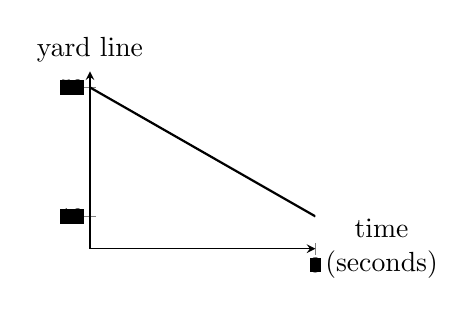
\begin{tikzpicture}
          \begin{axis}[ymin=0, xlabel style={align=center}, 
            xlabel={time\\(seconds)}, ylabel={yard line}, xtick={0, 
              3}, ytick={10, 50}, width=1.75in]
            \addplot[domain=0:3] { 50 - 40/3 * x};
          \end{axis}
        \end{tikzpicture} 
      \end{center}
    \end{solution}

  \item \label{function-football-not-function}

    \note{This problem is worded in a non-obvious way, but I hope that
      somebody will eventually hit on the idea that this graph says
      the ball can be in multiple places at once, which obviously
      doesn't make physical sense.}

    \begin{problem}[\vfill]
      Your friend Cris says, ``I was watching another football game on TV; one of the players had the ball and ran with it for a while before he got tackled!'' Cris draws the following graph to show you the ball's position during this play. Another friend, Lisa, says, ``I don't think that graph could possibly describe where the ball was!'' and asks you for your opinion. What do you think? How can you convince Cris and Lisa you're right?

      \begin{tikzpicture}
        \begin{axis}[xmin=0, xmax=8.25, ymin=0, xlabel
          style={align=center}, xlabel={time\\(seconds)}, ylabel={position\\(yard line)}, ylabel style={align=center}, width=2.5in]
          \addplot+[smooth] coordinates { (0, 40) (4.5, 30) (3.5, 
            25) (8, 15) }; %
          % \addplot[domain=5:40] ({8 - 2 * (x / 10 - 2)^2}, x); 
        \end{axis}
      \end{tikzpicture} 
    \end{problem}

    \begin{solution}
      What does this graph say about what's happening after, say, 4
      seconds? If we draw a vertical line at time 4, we see that it
      hits the graph in 3 places:
      \begin{center}
        \begin{tikzpicture}
          \begin{axis}[xmin=0, xmax=8.25, ymin=0, xlabel style={align=center}, xlabel={time\\(seconds)}, ylabel={position\\(yard line)}, ylabel style={align=center},, width=2.5in]
            \addplot+[smooth] coordinates { (0, 40) (4.5, 30) (3.5, 
              25) (8, 15) }; %
            \draw[gray] (4, 0) -- (4, 45); %
          \end{axis}
        \end{tikzpicture} 
      \end{center}
      But that says the ball is at 3 different yard lines at that
      single moment in time, which is of course impossible!
    \end{solution}
  \end{enumerate}

  \note{After students have had a chance to discuss \ref{function-football-pass} - \ref{function-football-not-function} with their groups, I'll bring the class together to discuss, and I'll introduce the language in the next box, as well as the vertical line test. }

  \begin{framed}
    \emph{Some important terminology!}
    \begin{itemize}[nosep]
    \item A \uline{function} is an input-output relationship with the key property that:
      \begin{center}
        For each possible input, \fitb{4in}{there is exactly 1 corresponding output}.
      \end{center}
      \begin{onehalfspace}
        Graphically, this means \fitb{4in}{the graph satisfies the vertical line test}. \solonly{(Read more about the vertical line test on pg. 32 of \robin{}.)}
      \end{onehalfspace}

    \item
      \begin{onehalfspace}
        The input variable is called the \fitb{1.5in}{independent} variable, and the output variable is called the \fitb{1.5in}{dependent} variable.%
      \end{onehalfspace}

    \item
      \begin{onehalfspace}
        When we graph a function, we put the \fitb{1.5in}{independent / input} variable on the horizontal axis and the \fitb{1.5in}{dependent / output} variable on the vertical axis.
      \end{onehalfspace}

    \item
      \begin{onehalfspace}
        The \uline{domain} of a function is the set of all \fitb{1in}{inputs}, and the \uline{range} is the set of all \fitb{1in}{outputs}.
      \end{onehalfspace}

    \end{itemize}
  \end{framed}

  \begin{enumerate}[resume]
  \item

    \note{I'll give students a moment to try this individually, and we'll talk about it. If I remember, I'll have them look back at the first 2 learning objectives to see that we've now discussed those.

    For domain and range, it's good to discuss the interval notation $[0, 3]$ just to make sure everyone understands it.}

    \begin{problem}[\vfill\newpage]
      Look back at the function in \ref{function-football-pass}, and
      identify the:
      \begin{itemize}
      \item independent variable
      \item dependent variable
      \item domain
      \item range
      \end{itemize}
    \end{problem}

    \begin{solution}
      The independent variable is time, the dependent variable is the
      yard line, the domain is $[0, 3]$, and the range is $[10, 50]$.
    \end{solution}

  \end{enumerate}

\item  \label{harvard-yard-chairs}  

  \begin{minipage}[t]{1.0\linewidth-1.65in}
    Harvard is ordering more colorful chairs for Harvard Yard. According to \href{https://www.thecrimson.com/flyby/article/2020/5/13/flyby-investigates-yard-chairs/}{Flyby}, the chairs cost \$381 each, with a minimum order of 2 chairs. Let $C(n)$ be the cost to buy $n$ chairs.
    \begin{enumerate}
    \item

      \note{Note on notation: Technically, $C$ is the function and $C(n)$ is the output when the input is $n$. But this distinction is meaningless to most students, so we won't try to make it. We will use all of the following when talking about functions: ``the function $f(x)$'', ``the function $f$'', ``the function $x^2$''.}

      \begin{problem}[0.75in]
        Is $C$ a function of $n$? Why or why not?
      \end{problem}

      \begin{solution}
        Yes: for each possible number of chairs, there is exactly one cost.
      \end{solution}

    \item

      \note{We aren't told whether there's a maximum number of chairs that can be ordered, so we don't have enough information to say what the domain is exactly. We'll talk about how, when we model real-world situations, we often need to make assumptions and choices.

        One issue that may come up here is whether we should model the domain  as a discrete set of values or a continuous one (and similarly for the range). If it does, we'll talk about how that's also a choice the modeler gets to make. }

      \begin{problem}[0.75in]
        What can you say about the domain of $C$?
      \end{problem}
    \end{enumerate}
  \end{minipage}
  \begin{minipage}[t]{1.6in}
    \vspace{-8pt}
    % https://www.fermob.com/en/Products/Furniture/Dining-chairs/Chairs-dining-armchairs/chair-luxembourg
    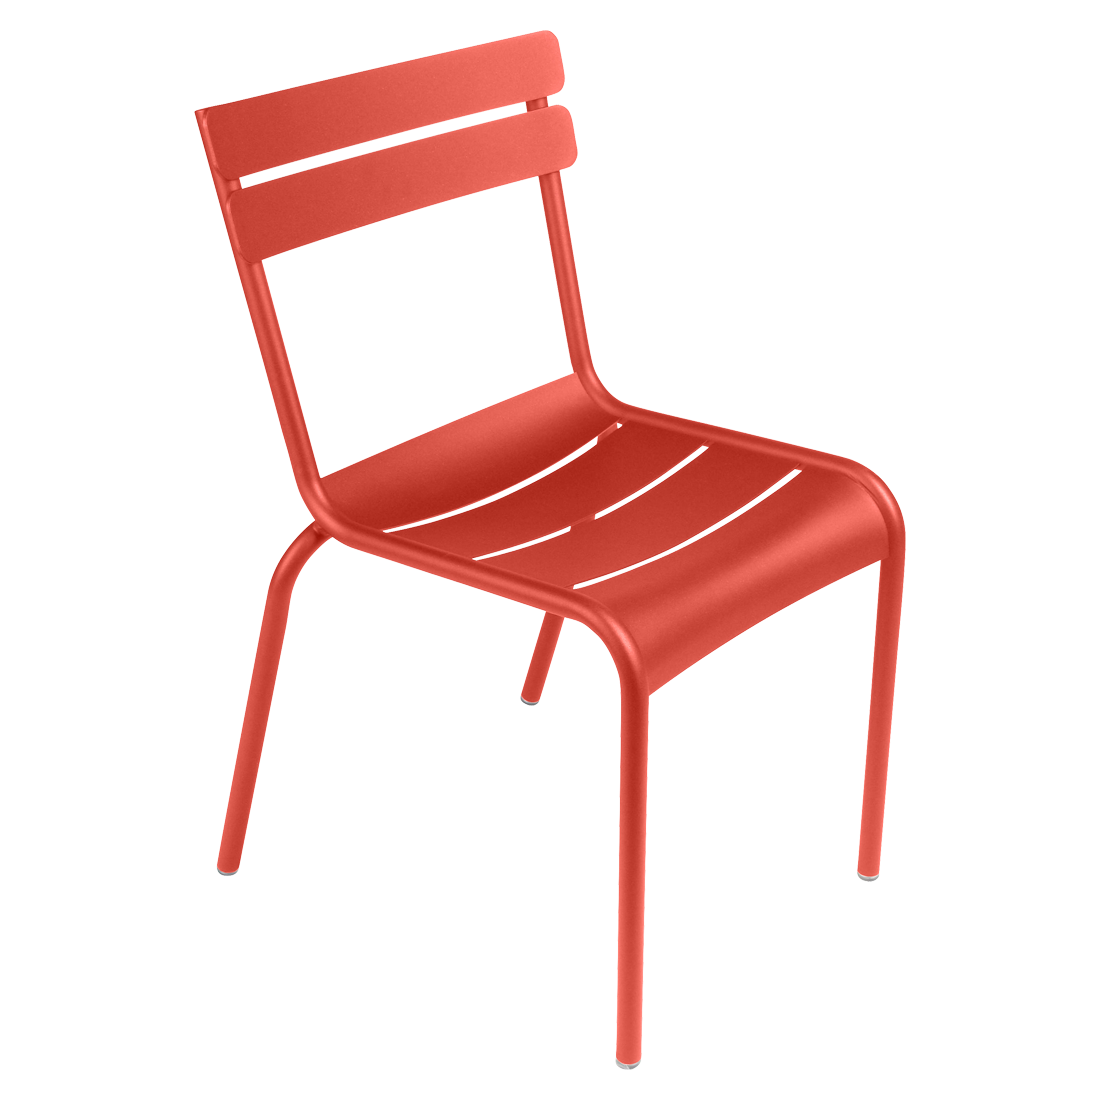
\includegraphics[width=1.5in]{images/fermob.png}
  \end{minipage}

  \begin{enumerate}[start=3]
  \item[]
    \begin{solution}
      We know Harvard must buy at least 2 chairs, but we aren't told whether there's a maximum number of chairs they can buy. So, we can't determine the domain exactly.

      It often happens when we're modeling that we don't have complete information about a situation, so we need to make some choices. Here, we could make the domain $\{2, 3, 4, 5, \ldots\}$, or we could make up a maximum number of chairs. For example, we can be pretty sure that Harvard won't buy more than 100000 chairs, so we could make the domain $\{2, 3, 4, 5, \ldots, 100000\}$.

      We say that our domain is \emph{discrete}, meaning that the values in the domain are separate (you can buy 2 chairs or 3 chairs, but you can't buy 2.5 chairs).

      We could, however, decide that we don't want our model to worry about this; in that case, we might choose to model using a \emph{continuous} domain $n \geq 2$. (In this model, $n = 2.5$ would be fine.) Even though this isn't strictly accurate, it's often useful to do this when building models, as it will enable us to use the tools of calculus to analyze our models.
    \end{solution}

  \item

    \note{There are two important points here:
      \begin{itemize}
      \item If we haven't talked about discrete vs. continuous already, we'll definitely talk about it here. I want students to understand that, in reality, this is a discrete situation (both chairs and money are discrete quantities), and the graph of that discrete situation is a bunch of dots. But in calculus, we often connect these into a continuous model (I'll stick with intuition here; ``continuous'' today just means we don't need to pick up our chalk when we draw the graph) because the tools of calculus that we'll learn are most useful for dealing with continuous functions.

        If students are very skeptical, I may also point out that, if we're interested in the overall trend of this function and we zoom out on the graph, it basically looks like a continuous line. Here's a Desmos graph that illustrates this: \url{https://www.desmos.com/calculator/snzgc7zpqb} And I might mention that this is common practice in many fields; economists often treat money as a continuous quantity even though you can't pay half a cent for something; biologists treat population as a continuous quantity even though you can't have half an animal; etc.

      \item The graph is linear, which happens because each additional chair causes the same increase in cost.

        A linear function has a slope, which is $\dfrac{\text{rise}}{\text{run}}$; in this case, we can think of that slope as being $\dfrac{\$381}{\text{1 chair}} = \$381$ per chair. (In particular, the slope is a \emph{rate}.)

      \end{itemize}
      If I remember, I'll have students look back at the third learning objective. 
    } 

    \begin{problem}[\vfill\newpage]
      Sketch the graph of $C$, and explain how you came up with your graph.
    \end{problem}

    \begin{solution}
      First, let's work with our \emph{discrete} model, where you aren't allowed to buy part of a chair.

      Each chair costs \$381, so if Harvard orders 2 chairs, it will cost $2 \cdot 381 = 762$ dollars. \textcolor{skyblue}{Adding 1 more chair} (represented by moving right by 1) \textcolor{hotpink}{adds \$381 dollars to the cost} (represented by moving up \$381). So, here's a graph showing the cost of 2 or 3 chairs.
      \begin{center}
        \begin{tikzpicture}
          \begin{axis}[xmin=0, ymin=0, xtick={1, 2, 3}, ytick={381, 762, ..., 10000}, clip=false, xlabel={chairs}, ylabel={cost (dollars)}]
            \draw[skyblue] (2, 762) -- node[below, text width=0.75in, 
            align=center]{Adding 1 more chair...} (3, 762); %
            \draw[hotpink] (3, 762) -- node[right, text width=0.75in, 
            align=center]{...makes the cost go up by \$381} (3, 1143);%
            \addplot+[closed] coordinates {(2, 762) (3, 1143) }; %
          \end{axis}
        \end{tikzpicture}
      \end{center}
      Each time we \textcolor{skyblue}{add 1 chair}, \textcolor{hotpink}{the cost goes up by \$381}:
      \begin{center}
        \begin{tikzpicture}
          \begin{axis}[xmin=0, ymin=0, xtick={1, 2, 3, 4, 5}, ytick={381, 762, ..., 10000}, xlabel={chairs}, ylabel={cost (dollars)}]            
            \draw[skyblue] (2, 762) -- (3, 762); %
            \draw[skyblue] (3, 1143) -- (4, 1143); %
            \draw[skyblue] (4, 1524) -- (5, 1524); %
            \draw[hotpink] (3, 762) -- (3, 1143); %
            \draw[hotpink] (4, 1143) -- (4, 1524); %
            \draw[hotpink] (5, 1524) -- (5, 1905); %
            \addplot+[closed] coordinates {(2, 762) (3, 1143) (4, 1524) (5, 1905) }; %
          \end{axis}
        \end{tikzpicture}
      \end{center}
      So, our discrete model ends up being a bunch of dots that all lie along a line:
      \begin{center}
        \begin{tikzpicture}
          \begin{axis}[xmin=0, ymin=0, xtick={1, 2, 3, 4, 5, ..., 10}, 
            ytick={381, 762, ..., 10000}, xlabel={chairs}, 
            ylabel={cost (dollars)}, title={Discrete model}]
            \addplot+[only marks, domain=2:10, samples=9]{381*x};
          \end{axis}
        \end{tikzpicture}
      \end{center}
      In contrast, our \emph{continuous} model would connect up the points:
      \begin{center}
        \begin{tikzpicture}
          \begin{axis}[xmin=0, ymin=0, xtick={1, 2, 3, 4, 5, ..., 10}, ytick={381, 762, ..., 10000}, xlabel={chairs}, ylabel={cost (dollars)}, title={Continuous model}]
            \addplot+[domain=2:10]{381*x};
          \end{axis}
        \end{tikzpicture}
      \end{center}      
    \end{solution}

  \end{enumerate}

\item  \label{martini-glass} 

  \note{The point of this problem is to have a non-linear example and to introduce concavity. If students are stuck, I will point out that, in the previous example, we thought about how each additional chair added to the cost. Here, we could similarly think of repeatedly adding a small amount of volume and see what that does to the height.

    Here, we get a graph that isn't linear, so it curves. We categorize how graphs curve using the words \emph{concave up} and \emph{concave down}.

    This problem is the last one I feel like we definitely need to cover in today's class. The remaining problems are more practice with thinking about concavity (in particular how concavity relates to rates of change). I hope there's time for students to try some of these, but it's totally okay if there isn't. }

  \begin{minipage}[t]{1.0\linewidth-1.1in-5pt}
    \setlength{\parskip}{8pt}
    \begin{problem}
      \href{https://journals.plos.org/plosone/article?id=10.1371/journal.pone.0204562}{A study} has found that the shape of a glass affects how quickly people drink from it. This happens because people have trouble judging how the volume of liquid in a non-cylindrical glass relates to the height of the liquid.

      Imagine you're pouring liquid into the glass shown to the right. Which of the following shows the height of the liquid as a function of the volume? Explain your choice.
    \end{problem}
  \end{minipage}
  \hspace{0.1in}
  \begin{minipage}[t]{1in}
    \vspace{-8pt}
    % https://www.amazon.com/Libbey-Cosmopolitan-Martini-Glasses-Set/dp/B01ESOCNTY/ref=psdc_13162311_t2_B097CH55HJ
    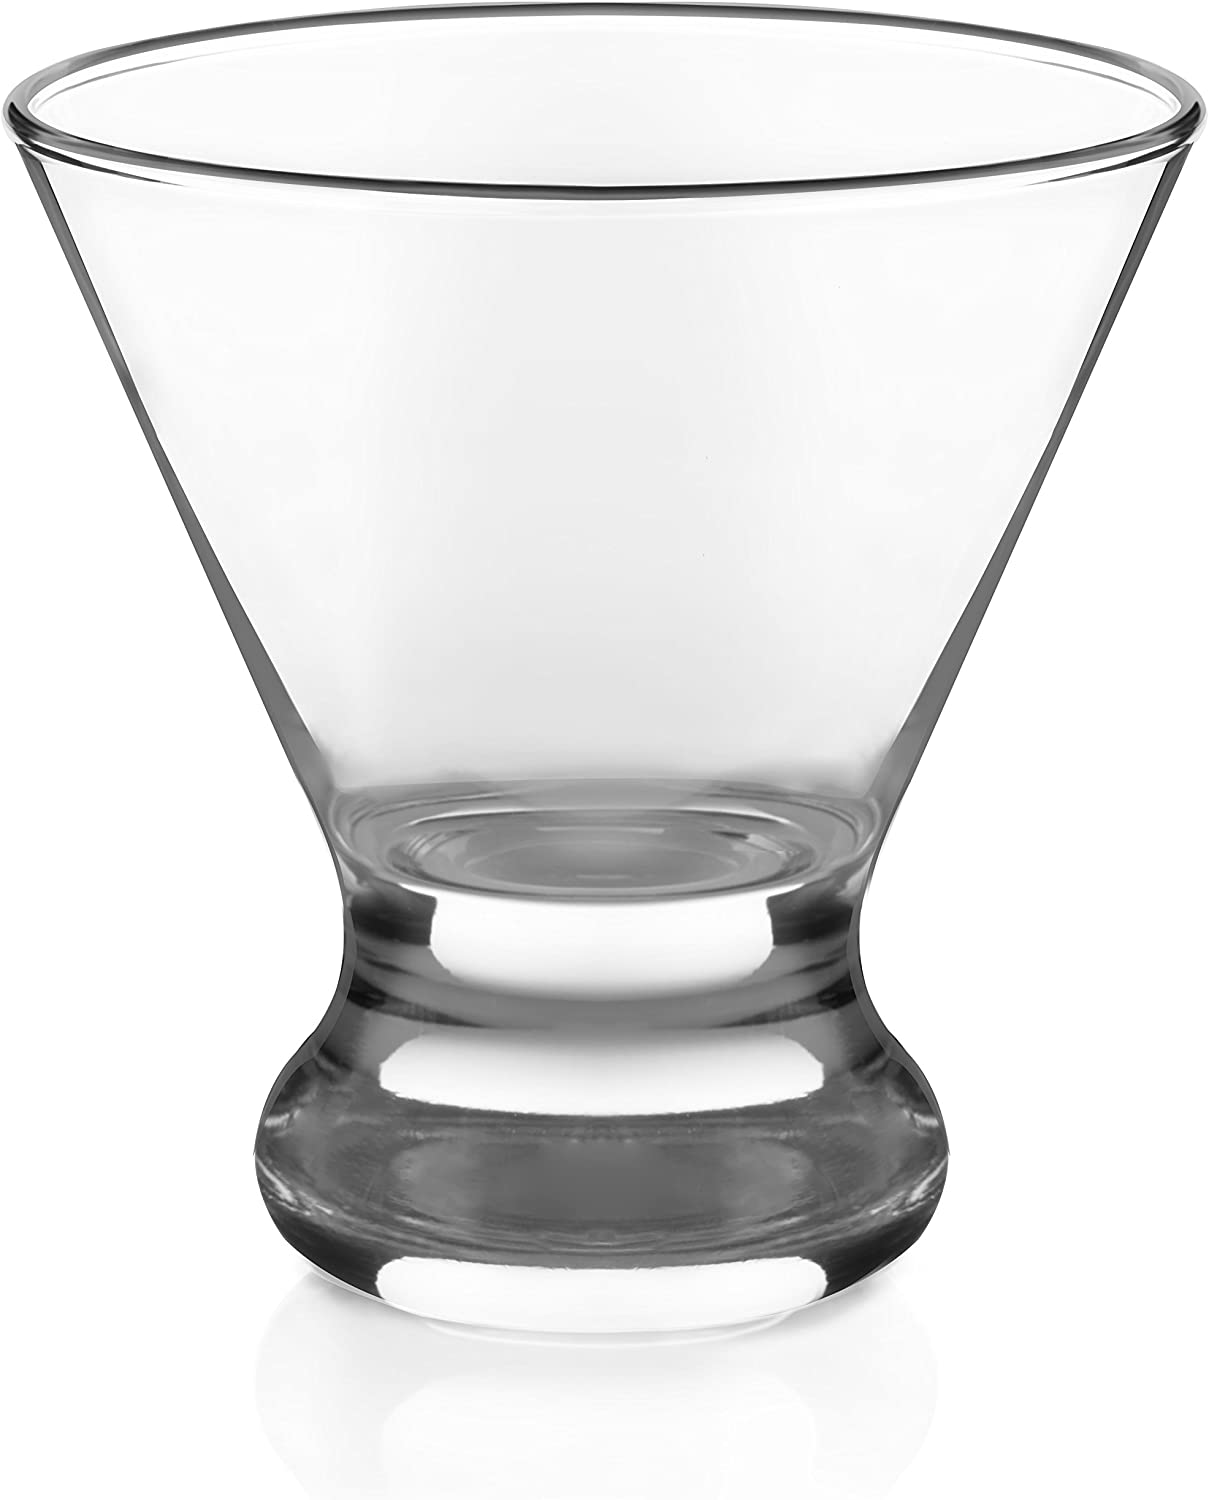
\includegraphics[width=0.8in]{images/martini-glass}    
  \end{minipage}

  \begin{problem}[\vfill]
    \begin{imagetable}{3}{\Alph}
      \begin{tikzpicture}
        \begin{axis}[width=1.75in, xtick=\empty, ytick=\empty]
          \addplot+[domain=0:4]{x / 2};
        \end{axis}
      \end{tikzpicture} &
      \begin{tikzpicture}
        \begin{axis}[width=1.75in, xtick=\empty, ytick=\empty]
          \addplot+[domain=0:7]{(1 + x)^(1/3) - 1};
        \end{axis}
      \end{tikzpicture} &
      \begin{tikzpicture}
        \begin{axis}[width=1.75in, xtick=\empty, ytick=\empty]
          \addplot+[domain=0:4]{x + x^2/3 + x^3/27};
        \end{axis}
      \end{tikzpicture}
    \end{imagetable}
  \end{problem}

  \begin{solution}
    In \ref{harvard-yard-chairs}, we thought about how adding 1 chair at a time affected the cost. Here, we're dealing with a continuous quantity, but we can use a similar strategy. Imagine we repeatedly add a tiny amount of water to the glass, like 1 teaspoon at a time. The first teaspoon will increase the height of the liquid in the glass from 0 to some small height. If we add a second teaspoon, the height will again increase, but by less than before because the glass is wider, so the second teaspoon ``spreads out'' more. Here's a diagram:
    \begin{center}
      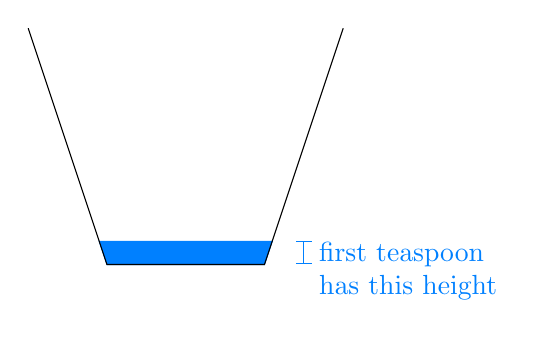
\begin{tikzpicture}
        \filldraw[skyblue] (-1.1, 0.3) -- (-1, 0) -- (1, 0) -- (1.1, 
        0.3); %
        \draw (-2, 3) -- (-1, 0) -- (1, 0) -- (2, 3); %
        \draw[|-|, skyblue] (1.5, 0) -- (1.5, 0.3) node[anchor=north
        west, text width=0.9in, xshift=2pt, yshift=3pt]{first teaspoon has this height} ; %
      \end{tikzpicture}
      \qquad
      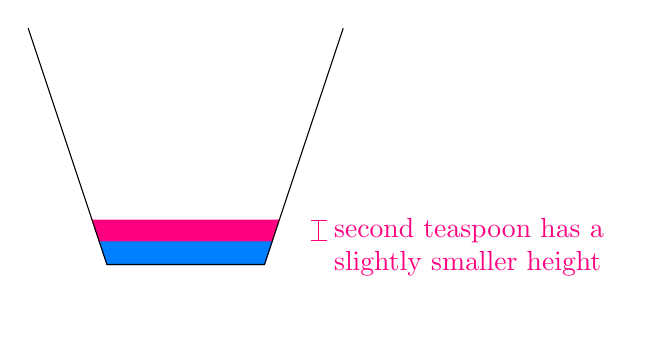
\begin{tikzpicture}
        \filldraw[skyblue] (-1.1, 0.3) -- (-1, 0) -- (1, 0) -- (1.1, 
        0.3); %
        \filldraw[hotpink] (-1.19, 0.57) -- (-1.1, 0.3) -- (1.1, 
        0.3) -- (1.18, 0.57); %
        \draw (-2, 3) -- (-1, 0) -- (1, 0) -- (2, 3); %
        \draw[|-|, opacity=0] (1.5, 0) -- (1.5, 0.3) node[anchor=north
        west, text width=0.9in, xshift=2pt, yshift=3pt]{first teaspoon has this height} ; %
        \draw[|-|, hotpink] (1.69, 0.3) -- (1.69, 0.57) node[anchor=north
        west, text width=1.5in, xshift=2pt, yshift=4pt]{second teaspoon
          has a slightly smaller height} ; %        
      \end{tikzpicture}
    \end{center}
    The two pictures above correspond to these two points on the graph
    of height vs.\ liquid:
    \begin{center}
      \begin{tikzpicture}
        \begin{axis}[xlabel={volume}, ylabel={height}, xmin=0, ymin=0, 
          xtick=\empty, ytick=\empty, clip=false]
          \draw[skyblue, thick] (0, 0) -- node[below]{1 teaspoon} (1, 
          0) -- node[right, text width=0.9in]{height of first
            teaspoon} (1, 0.3); %
          \draw[hotpink, thick] (1, 0.3) -- node[below]{1 teaspoon} (2, 
          0.3) -- node[right, text width=1in]{height of second
            teaspoon} (2, 0.57); %
          \addplot+[closed] coordinates { (0, 0) (1, 0.3) (2, 0.57) }; 
        \end{axis}
      \end{tikzpicture}
    \end{center}
    Since the glass keeps getting wider as we move up, each teaspoon
    will increase the height by less than the previous teaspoon.
    Therefore, if we keep plotting points in this way, we get a
    picture like this:
    \begin{center}
      \begin{tikzpicture}
        \begin{axis}[xlabel={volume}, ylabel={height}, xmin=0, ymin=0, 
          xtick=\empty, ytick=\empty, clip=false]
          \addplot+[only marks, domain=0:10, samples=11] {(1 +
            x)^(1/3) - 1}; 
        \end{axis}
      \end{tikzpicture}
    \end{center}
    We haven't plotted what happens for every possible volume, but we can see enough of the trend to be sure that the correct graph is \fbox{(B)}.
  \end{solution}

\item  \label{connally-2.5.14} 

  After a cup of hot chocolate is poured, the temperature cools off very rapidly at first, and then cools off more slowly, until the temperature of the hot chocolate eventually reaches room temperature. Let $H(t)$ be the hot chocolate's temperature in $^\circ$F $t$ minutes after it's been poured.

  \begin{enumerate}
  \item
    \begin{problem}[\stretch{0.75}]
      Sketch a graph of $H(t)$. 
    \end{problem}

    \begin{solution}
      We can use the same strategy as in \ref{martini-glass}. This time, we'll think about what happens each minute. The hot chocolate is cooling off, so its temperature is decreasing.

      In the first minute, the temperature decreases by some amount. We're told that the hot chocolate cools off more slowly as time goes on; therefore, in each minute, the temperature will decrease by a smaller amount than in the minute before. If we think of plotting one temperature reading per minute, we can see that those would look something like this:
      \begin{center}
        \begin{tikzpicture}
          \begin{axis}[xmin=0, ymin=0, xtick=\empty, ytick=\empty, 
            xlabel=$t$, ylabel=temperature]
            \addplot+[domain=0:10, samples=11, only marks] {70 + 50 * 1.3^(-x)};
          \end{axis}
        \end{tikzpicture}
      \end{center}
      So, we can see that the graph of $H(t)$ should be concave up. We're also told that the temperature should eventually reach room temperature, and we can infer that it should stay at room temperature after that. So, the entire graph really looks something like this:
      \begin{center}
        \begin{tikzpicture}
          \begin{axis}[xmin=0, ymin=0, xtick=\empty, ytick=\empty, xlabel=$t$, ylabel=temperature, ytick={70}, yticklabels={room temperature}]
            \addplot+[domain=0:25] {70 + 50 * 1.3^(-x)};
          \end{axis}
        \end{tikzpicture}
      \end{center}
    \end{solution}

  \item
    \begin{problem}[\nstretch{0.25}]
      Is $H$ increasing, decreasing, or constant? Is $H$ concave up, concave down, or linear?
    \end{problem}

    \begin{solution}
      Decreasing and concave up.
    \end{solution}

  \end{enumerate}

\item  
  \begin{problem}[\vfill]
    According to a \href{https://people.math.harvard.edu/~jjchen/mathma/docs/articles/22carbon.html}{New York Times article on the level of carbon dioxide in the atmosphere}, ``not only is the carbon dioxide level rising relentlessly, but the pace of that rise is accelerating over time.'' What does this tell you about the graph of carbon dioxide level as a function of time?
  \end{problem}

  \begin{solution}
    Using the same reasoning as in \ref{martini-glass} and
    \ref{connally-2.5.14}, we find that the graph is increasing and
    concave up. 
  \end{solution}

\item   % QRD

  % Data sources:
      % https://www.census.gov/history/pdf/1978tvsets.pdf and https://www2.census.gov/library/publications/2008/compendia/statab/128ed/tables/09s1090.xls

  \begin{problem}[\vfill]
    Here's a graph showing the number of millions of US households with a color television as a function of time.

    \begin{center}
      \begin{tikzpicture}
        \begin{axis}[xlabel={Year}, ylabel={Millions of households}]
          \addplot[smooth] file {data/color-tv.txt};
        \end{axis}
      \end{tikzpicture}
    \end{center}

    Based on this graph, narrate how color TVs were adopted in the US. (How did the rate at which households adopted color TVs change over time? When was it speeding up? When was it slowing down? Can you come up with some plausible reason for that?)
  \end{problem}

  \begin{solution}
    Until the early 1960s, the rate at which households were getting color TVs was very slow. This rate sped up from about 1964 to the mid-1970s, then it seemed to be pretty steady until 1990. In the 1990s, the number of households with color TVs continued to increase, but at a slower rate than before.

    A plausible explanation is that, in the 1960s, color TVs were just becoming available, so the rate at which households adopted them increased. It held steady for a long time, but by the 1990s, most households had color TVs, so the rate at which households got them slowed down.
  \end{solution}

\end{enumerate}
\end{document}
